\documentclass[11pt]{article}
\usepackage{fullpage}
\usepackage{graphicx, subfigure}
\usepackage{parskip}

\title{Artificial Neural Nets for Face Detection}
\author{Rita Zevallos and Jacob Carstenson}
\usepackage{float}
\usepackage{filecontents}
\begin{filecontents}{bib}

@misc{mitchell1997machine,
  title={Machine learning. WCB},
  author={Mitchell, Tom M},
  year={1997},
  publisher={McGraw-Hill Boston, MA:}
}

@TechReport{fddbTech,
  author = {Vidit Jain and Erik Learned-Miller},
  title =  {FDDB: A Benchmark for Face Detection in Unconstrained Settings},
  institution =  {University of Massachusetts, Amherst},
  year = {2010},
  number = {UM-CS-2010-009}
  }
  
  \end{filecontents}
% for back reference in bibliography
\usepackage[style=alphabetic,citestyle=alphabetic,backend=biber,backref=true]{biblatex}
\addbibresource{bib}
\DeclareFieldFormat[inbook]{citetitle}{#1}
\DeclareFieldFormat[inbook]{title}{#1}

\begin{document}

\maketitle

\section{Introduction}



The problem we have chosen to tackle is the problem of detecting whether a face is in in an image. Originally we wanted to have pictures of varying dimensions and have the system give a bounding box around each face in the image, similar to what many modern cameras use to detect faces. This proved to be too hard of a problem so we had to modify our problem to detecting whether a 20 by 20 pixel image contains a face or not.

In order to tackle this problem, the machine learning technique we chose to use is an artificial neural network, created by the conx python module, part of the Pyrobotics project. Artificial neural networks are a generalized supervised learning approach inspired by biological processes in the brain \cite{mitchell1997machine}. This network contains artificial neurons, organized into three layers (input, hidden, output), that have a series of inputs that are linearly combined with an associated set of weights to produce its net input. The net input is passed into an activation function that produces this neuron's activation which is passed on to the inputs of the next layer. The activation function used in our neural network is a sigmoid function, which is a differentiable function that maps very negative numbers to 0 and very positive numbers to one and numbers that are exactly 0 are mapped to 0.5. The activations of the output layer nodes represent the answer the neural net gives.

This network is trained with input taken from our obtained dataset along with a set of target values we want the system to output, in this case the output should be either 1 for the image is a face or 0 for images without a face. However, adding a tolerance allows the system to categorize with more leniency: for example, a tolerance of 0.2 allows images with activation from 0.0 to 0.2 to be categorized as not faces, and image with activation from 0.8 to 1.0 to be categorized as faces.


\section{Details}

\subsection{Dataset and Preprocessing}


We constructed our dataset from the Face Detection Data Set and Benchmark (FDDB)\cite{fddbTech}, a set of 2845 images of different dimensions taken from news photographs. The set comes with files that define annotations locating a bounding ellipse for each face in each of the images. See Figure \ref{fig:sample_ellipse} for an example such annotation.
 \begin{figure}[H]
     \begin{center}
%
        \subfigure[]{%
            \label{fig:sample_ellipse}
            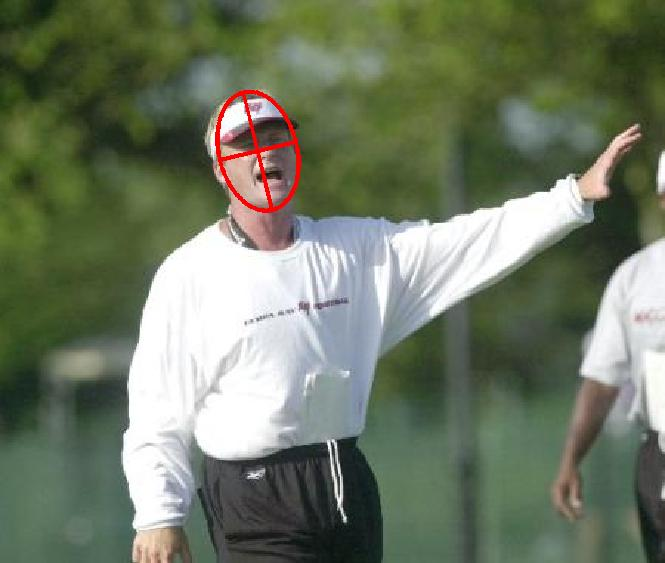
\includegraphics[width=0.4\textwidth]{screenshots/example_ellipse.jpg}
        }\\%
        \subfigure[]{%
            \label{fig:sample_face}
            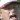
\includegraphics[width=0.2\textwidth]{screenshots/example_baseball.jpg}
        }%
        \subfigure[]{%
            \label{fig:sample_face_rgb}
            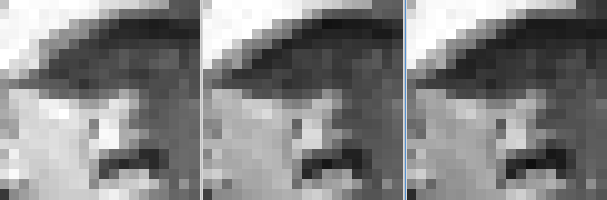
\includegraphics[width=0.4\textwidth]{screenshots/example_face_rgb.png}
        }\\%
        \subfigure[]{%
            \label{fig:sample_notface}
            
\includegraphics[width=0.2\textwidth]{screenshots/example_not_color.png}
        }%
        \subfigure[]{%
            \label{fig:sample_notface_rgb}
            
\includegraphics[width=0.4\textwidth]{screenshots/example_not_rgb.png}
        }\\%
    \end{center}
    \caption{%
        The dataset preprocessing procedure: (1) Choose images from the original dataset that contain only one face (2) Extract a 20x20 square containing a face and a 20x20 square not containing a face (3) Separate into the RGB channels to input into the neural net.
     }\label{fig:notface}%
\end{figure}


From a subset of these images, we cropped to squares inside (see Figure \ref{fig:sample_face}) and outside (see Figure \ref{fig:sample_notface} of these ellipses, resulting of a dataset of 1358 square images, 679 of which contain faces and 679 of which do not contain faces. These squares were then resized to 20 by 20 pixel images, decreasing the resolution significantly.


We converted all the images to the PPM (Portable Pixmap) format, a lossless image format which contains an array of bytes, each a decimal value between 0 and 255 that represent the individual red, green, and blue values of each pixel. See Figures \ref{fig:sample_face_rgb} and \ref{fig:sample_notface_rgb} for examples of the original images separated into the three color channels. We used the Python Imaging Library (PIL) for the cropping and converting of each image from the FDDB database.

These PPM images are imported to the Pyrobot vision module that stores all of the RGB values and normalizes the values between 0 and 1. The values are then written in ASCII to an inputs.dat file where each line of the file contains every RGB value of a 20 by 20 image separated by spaces. Each line of the file will then represent the 1200 input nodes for the neural network. Since we had 1358 images, the inputs.dat file had 1358 lines.

Another file corresponding to the inputs.dat file is the targets.dat file. Each image contained within the inputs.dat file is mapped to an integer value representing whether the image is a face (1) or not a face (0). This file represents what we want the neural network to produce when presented with these images.

\subsection{Neural Network}

The software defining the artificial neural network was written in python and obtained from the Python Robotics programming environment.

We used a network with 1200 input nodes (400 pixels, 3 color values for each pixel), a single hidden layer with 200 hidden nodes, and 1 output node.

Since the neural net recieves each image as RGB seperated values, we chose to grab every third value and visualize it as a 20 by 20 array. This way when showing the performance of the neural net, three images of the seperated RGB values of the image are depicted allong with the hidden and output layer activations

We used 80\%, or 1087 images, of the data as the training data, and 20\%, or 271 images, as the test data. The data was split randomly into the two sets for each run.


The training parameters were as following:

\begin{table}[h]
\begin{tabular}{ll}
Learning rate & 0.05  \\
Momentum      & 0.0 \\
Report rate   & 1    \\
Tolerance     & 0.35
\end{tabular}
\end{table}

We trained for one epoch at a time and then evaluated on the test set, stopping when performance decreased on the test set, to prevent over-training. This would usually take between 5 and 7 epochs.

\section{Results}


The scores on both the training set and the test set are shown in Figure \ref{fig:performance_graph}, in terms of the percent labeled correctly as faces or not faces.

\begin{figure}[h]
    \centering
    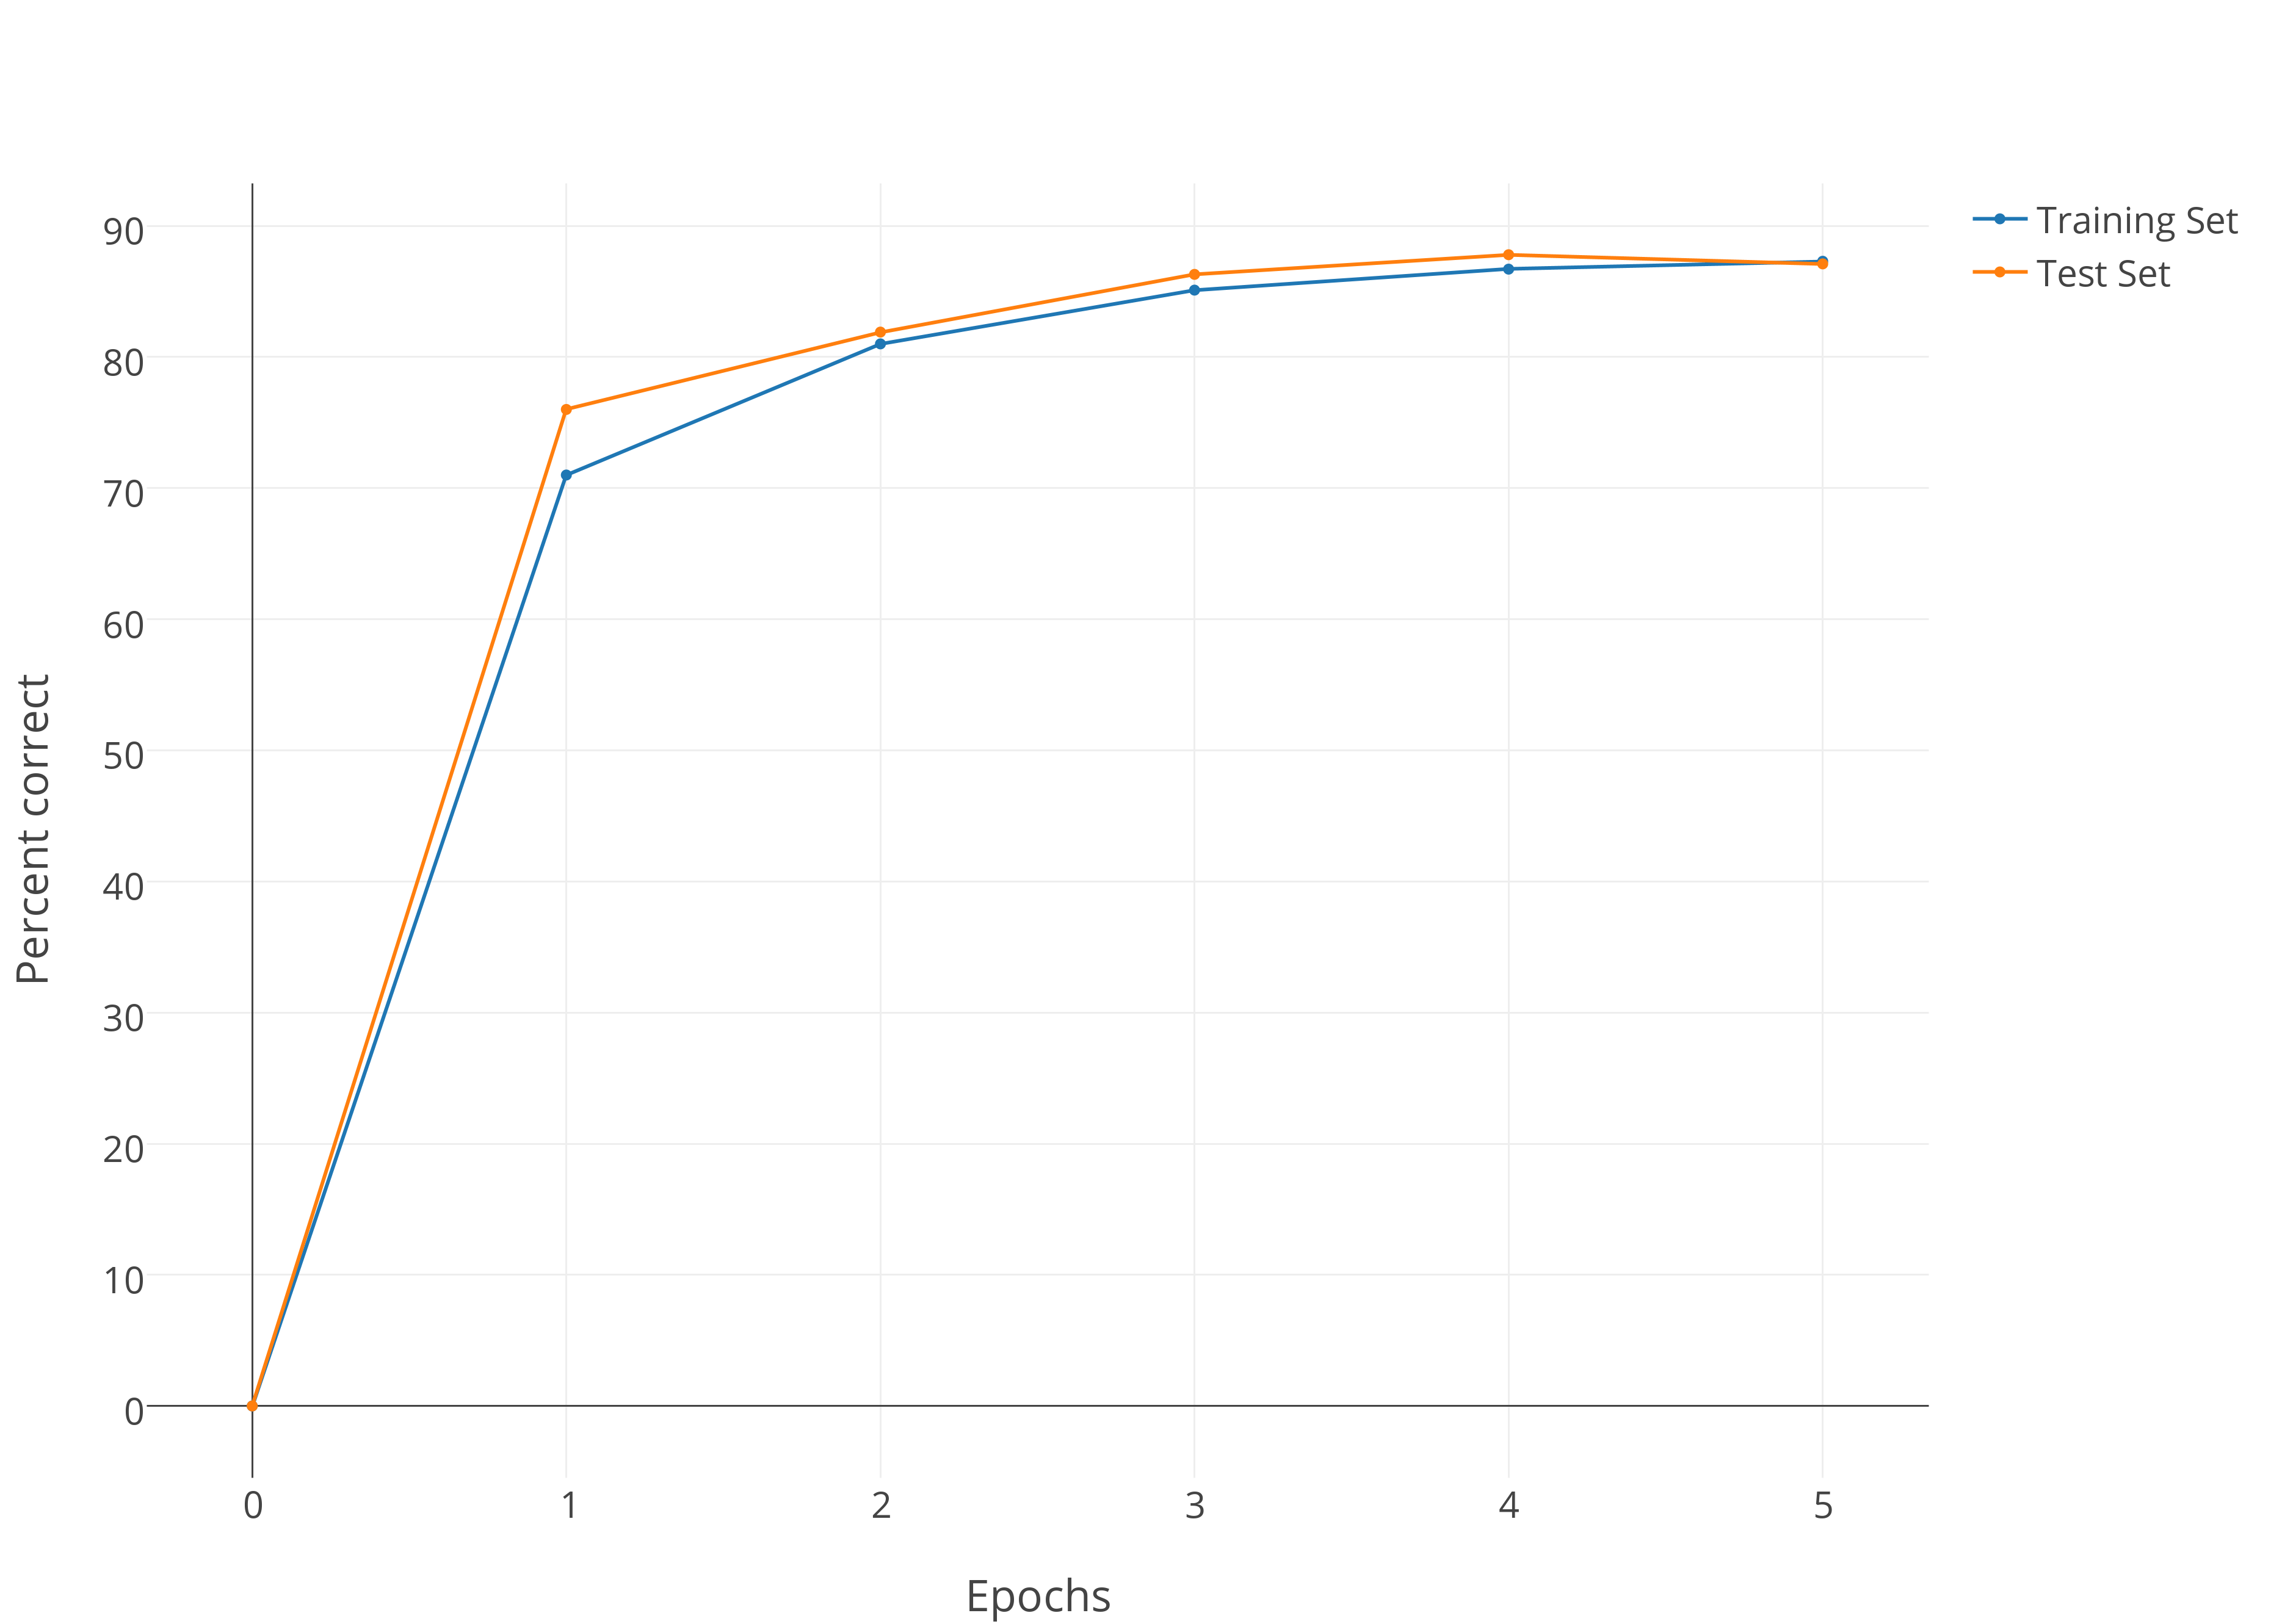
\includegraphics[width=0.8\textwidth]{performance_graph.png}
    \caption{Performance graph}
    \label{fig:performance_graph}
\end{figure}
The neural net reached an accuracy of 87.8\% correctly categorized images of the test set.

There were several interesting cases among the images that were labeled incorrectly which give light on the pitfalls of our trained neural network.

 \begin{enumerate} 
 \item \textit{Rotated faces.} The neural net failed to categorize some faces where the angle of rotation was significant. See Figure \ref{fig:rotated_face} for an example. This could be because most of the training set is unrotated.
 \item \textit{Cut off faces. } This is a problem that came about from our preprocessing which took cropped squares acording to the face annotation supplied from the FDDB. Some pictures, such as Figure \ref{fig:cutoff_face} did not include the mouth and/or chin of the subject. Some of these images were incorrectly categorized as not faces.
 \item \textit{Clothing/obstructions. } Faces that were obstructed by sunglasses, hats, or facial hair, such as Figure \ref{fig:obstruction_face} were often categorized incorrectly.
 \item \textit{Skin tone.}  Most of the faces in the FDDB dataset were light-skinned. Dark-skinned people, such as \ref{fig:skintone_face} were often categorized incorrectly. This could be solved by finding a more diverse dataset.
 \item \textit{Open mouth. } Most of the subjects in the training set had their mouths closed. Faces with mouths open, such as \ref{fig:openmouth_face} were often categorized incorrectly. This could be because while a closed mouth is dark on the face, an open mouth showing teeth is fairly white.
 \item \textit{Lighting issues. } There was some bad data, such as in Figure \ref{fig:lighting_face}, where the faces were too blurry or badly lighted to be identified.
 \end{enumerate}
 
 
  \begin{figure}[ht!]
     \begin{center}
%
        \subfigure[Rotated face. Activation 0.55]{%
            \label{fig:rotated_face}
            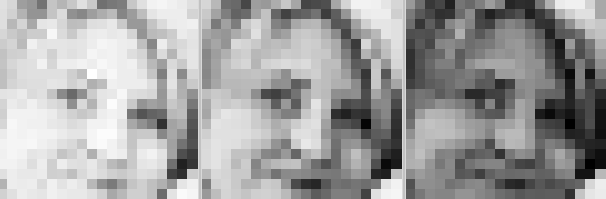
\includegraphics[width=0.4\textwidth]{screenshots/face_rotated_55.png}
        }%
        \subfigure[Cut off face. Activation 0.52]{%
            \label{fig:cutoff_face}
            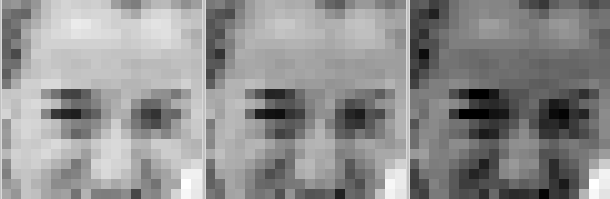
\includegraphics[width=0.4\textwidth]{screenshots/face_cropped_lookingdown_52.png}
        }\\%
        \subfigure[Face obstruction. Activation 0.40]{%
            \label{fig:obstruction_face}
            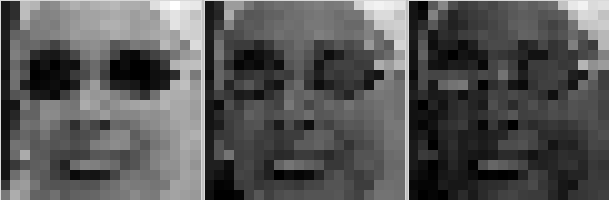
\includegraphics[width=0.4\textwidth]{screenshots/face_obstruction_sunglasses_40.png}
        }%
        \subfigure[Skin tone. Activation 0.14]{%
            \label{fig:skintone_face}
            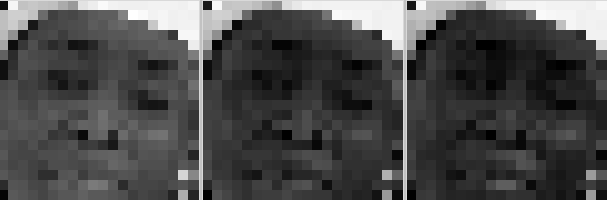
\includegraphics[width=0.4\textwidth]{screenshots/face_race_14.png}
        }\\%
        \subfigure[Open mouth. Activation 0.21]{%
            \label{fig:openmouth_face}
            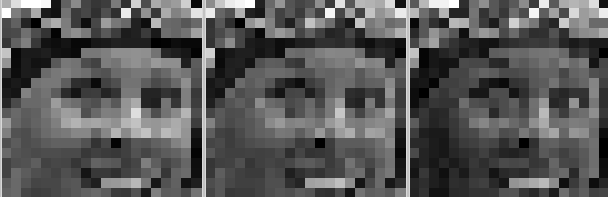
\includegraphics[width=0.4\textwidth]{screenshots/face_openmouth_21.png}
        }%
        \subfigure[Lighting issues. Activation 0.45]{%
            \label{fig:lighting_face}
            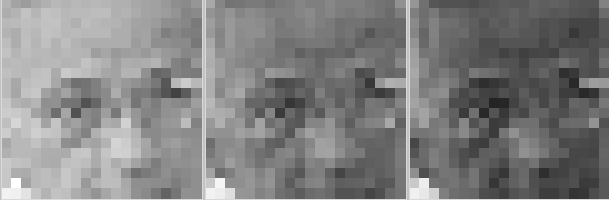
\includegraphics[width=0.4\textwidth]{screenshots/face_lighting_45.png}
        }%
    \end{center}
    \caption{%
        Examples of images containing faces that were incorrectly categorized as not containing faces. Activation shows the strength of the neural net's confidence. Because our tolerance was 0.35, activation scores between 0.0 and 0.35 were categorized as \textbf{'not face'}, activations between 0.65 and 1.0 were categorized as \textbf{'face'}, and activations between 0.36 and 0.64 were categorized as \textbf{'unknown'}.
     }%
\end{figure}

The photos that did not include faces that were incorrectly categorized as being faces were less easy to analyze for common features. However, we show some examples in Figure \ref{fig:notface}.
 
 \begin{figure}[ht!]
     \begin{center}
%
        \subfigure[Activation 0.79]{%
            \label{fig:notface1}
            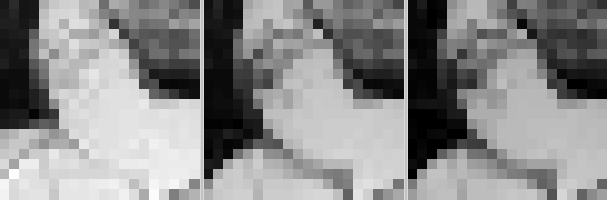
\includegraphics[width=0.4\textwidth]{screenshots/notface_idk_79.png}
        }%
        \subfigure[Activation 0.83]{%
            \label{fig:notface2}
            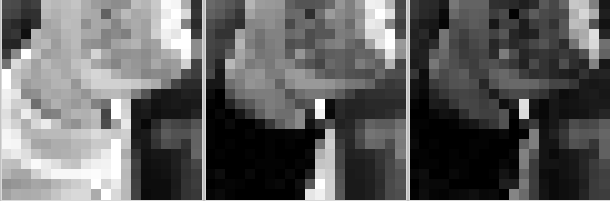
\includegraphics[width=0.4\textwidth]{screenshots/notface_necklike_83.png}
        }\\%
        \subfigure[Activation 0.43]{%
            \label{fig:notface2}
            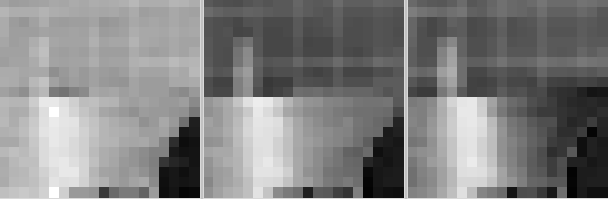
\includegraphics[width=0.4\textwidth]{screenshots/notface_pinky_43.png}
        }%
        \subfigure[Activation 0.70]{%
            \label{fig:notface2}
            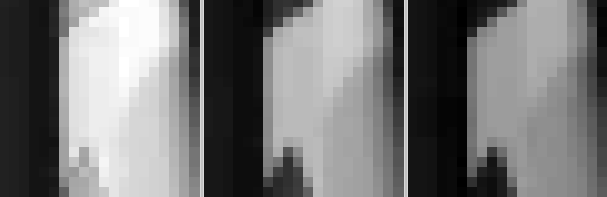
\includegraphics[width=0.4\textwidth]{screenshots/notface_waterfall_70.png}
        }\\%
    \end{center}
    \caption{%
        Examples of images not containing faces that were incorrectly categorized as faces. 
     }\ref{fig:notface}%
\end{figure}

\section{Conclusions and Future Work}

Our simple, 3-layer neural network performed well overall on the data set. Potential changes to our method in the future could include adjusting the input data, and adjusting our neural net.

With regards to the neural net, we could explore using multiple hidden layers, or creating different organizations of input, such as inputting rows or columns as sections.

While we chose to have our input data be in the simplest possible form, it could be interesting to try using different formats and color models for our input data. The Hue Saturation Value (HSV) color model is often used for computer vision problems instead of RGB because it isolates the color information (hue) from the intensity information. 

Also, instead of using raw pixel data as our inputs, it could be beneficial to extract feature vectors for each pixel that contain more information about that pixel in its local context.

We could also explore using different datasets. Many of the problems in incorrect categorizations resulted from the dataset being non-representative. Having a dataset that is more diverse and does not contain any badly cropped faces could solve these issues.

 \newpage
% bibliography
\printbibliography

\end{document}